\begin{figure}[t]
\centering
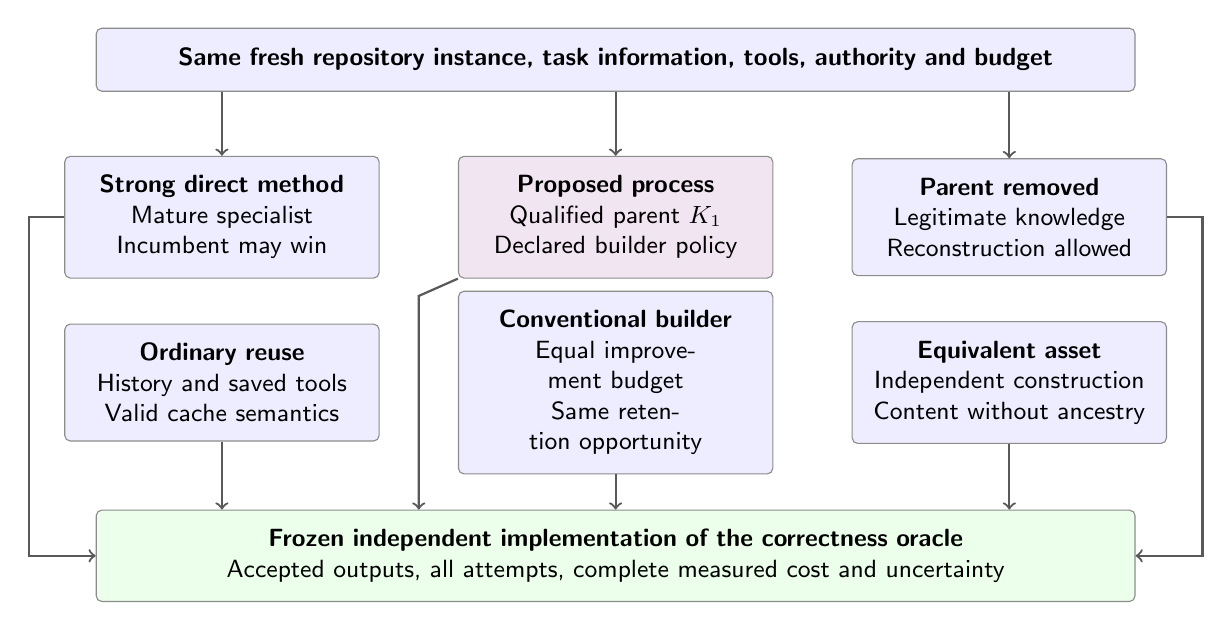
\begin{tikzpicture}[
  font=\sffamily\small,
  box/.style={draw=black!45, rounded corners=2pt, align=center, text width=3.5cm, minimum height=1.15cm, inner sep=7pt},
  flow/.style={->, thick, draw=black!65}
]
\node[box,fill=blue!7,text width=12.7cm,minimum height=0.8cm] (inputs) at (5,0) {\textbf{Same fresh repository instance, task information, tools, authority and budget}};
\node[box,fill=blue!7] (direct) at (0,-2) {\textbf{Strong direct method}\\Mature specialist\\Incumbent may win};
\node[box,fill=violet!10] (parent) at (5,-2) {\textbf{Proposed process}\\Qualified parent $K_1$\\Declared builder policy};
\node[box,fill=blue!7] (removed) at (10,-2) {\textbf{Parent removed}\\Legitimate knowledge\\Reconstruction allowed};
\node[box,fill=blue!7] (ordinary) at (0,-4.1) {\textbf{Ordinary reuse}\\History and saved tools\\Valid cache semantics};
\node[box,fill=blue!7] (conventional) at (5,-4.1) {\textbf{Conventional builder}\\Equal improvement budget\\Same retention opportunity};
\node[box,fill=blue!7] (equivalent) at (10,-4.1) {\textbf{Equivalent asset}\\Independent construction\\Content without ancestry};
\node[box,fill=green!8,text width=12.7cm,minimum height=1.0cm] (judge) at (5,-6.3) {\textbf{Frozen independent implementation of the correctness oracle}\\Accepted outputs, all attempts, complete measured cost and uncertainty};
\foreach \n in {direct,parent,removed}{\draw[flow] (inputs.south -| \n.north) -- (\n.north);}
\draw[flow] (direct.west) -- ++(-0.45,0) |- (judge.west);
\draw[flow] (parent.south west) -- (2.5,-3.0) -- (2.5,-5.2) -- (judge.north -| 2.5,0);
\draw[flow] (removed.east) -- ++(0.45,0) |- (judge.east);
\foreach \n in {ordinary,conventional,equivalent}{\draw[flow] (\n.south) -- (judge.north -| \n.south);}
\end{tikzpicture}
\caption{Causal comparison structure. Parent removal measures the value of ready executable content while permitting reconstruction. An equivalent asset distinguishes content from ancestry. Ordinary reuse and an equally funded conventional builder prevent attributing familiar engineering advantages to a new name. Repeated timings within an instance are subsamples, not additional independent missions.}
\label{fig:comparisons}
\end{figure}
